\chapter{Introduction}\label{ch:introduction}

The Standard Model of particle physics, which describes the fundamental constituents of matter and their interactions, represents an unambiguous triumph of the scientific method. Its predictions have been verified to extraordinary precision. The last missing piece of the standard model, the Higgs boson, was discovered in 2012, fifty years after it was predicted. This resulted in a Nobel prize for Francois Englert and Peter Higgs, and in much jubilation among the particle physics community. 

\begin{marginfigure}[2.5cm]
  \centering
  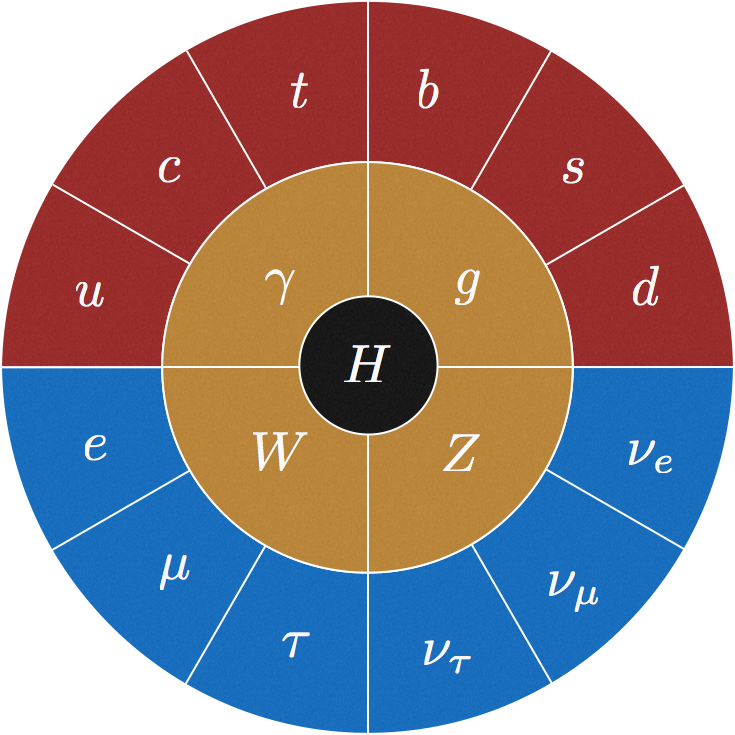
\includegraphics[width=0.8\textwidth]{images/SM-wheel.png}
  \caption{Graphical representation of the particle content of the standard model Source: the movie \emph{Particle Fever} (2013).}
\end{marginfigure}

However, many questions still remain unanswered by the standard model. On a very basic level, the standard model does not explain why neutrinos have masses, and does not have a viable dark matter candidate. On a more abstract level, the mass of the Higgs boson in the standard model is not protected from large radiative corrections, and seems unnaturally finely tuned - this is termed the \emph{hierarchy problem}. And perhaps the greatest challenge is that of reconciling the standard model with the theory of general relativity. In fact, it is widely believed that the Standard Model is only a low-energy effective approximation to an underlying theory that is valid at higher energy scales.

To answer these questions, we must go beyond the Standard Model with new theories. These new theories often predict new fundamental particles and forces. Currently, our best tools to study these new particles are particle colliders, like the Large Hadron Collider (LHC), which lies on the border between Switzerland and France (\autoref{fig:LHC_schematic}).

\begin{figure}
  \centering
  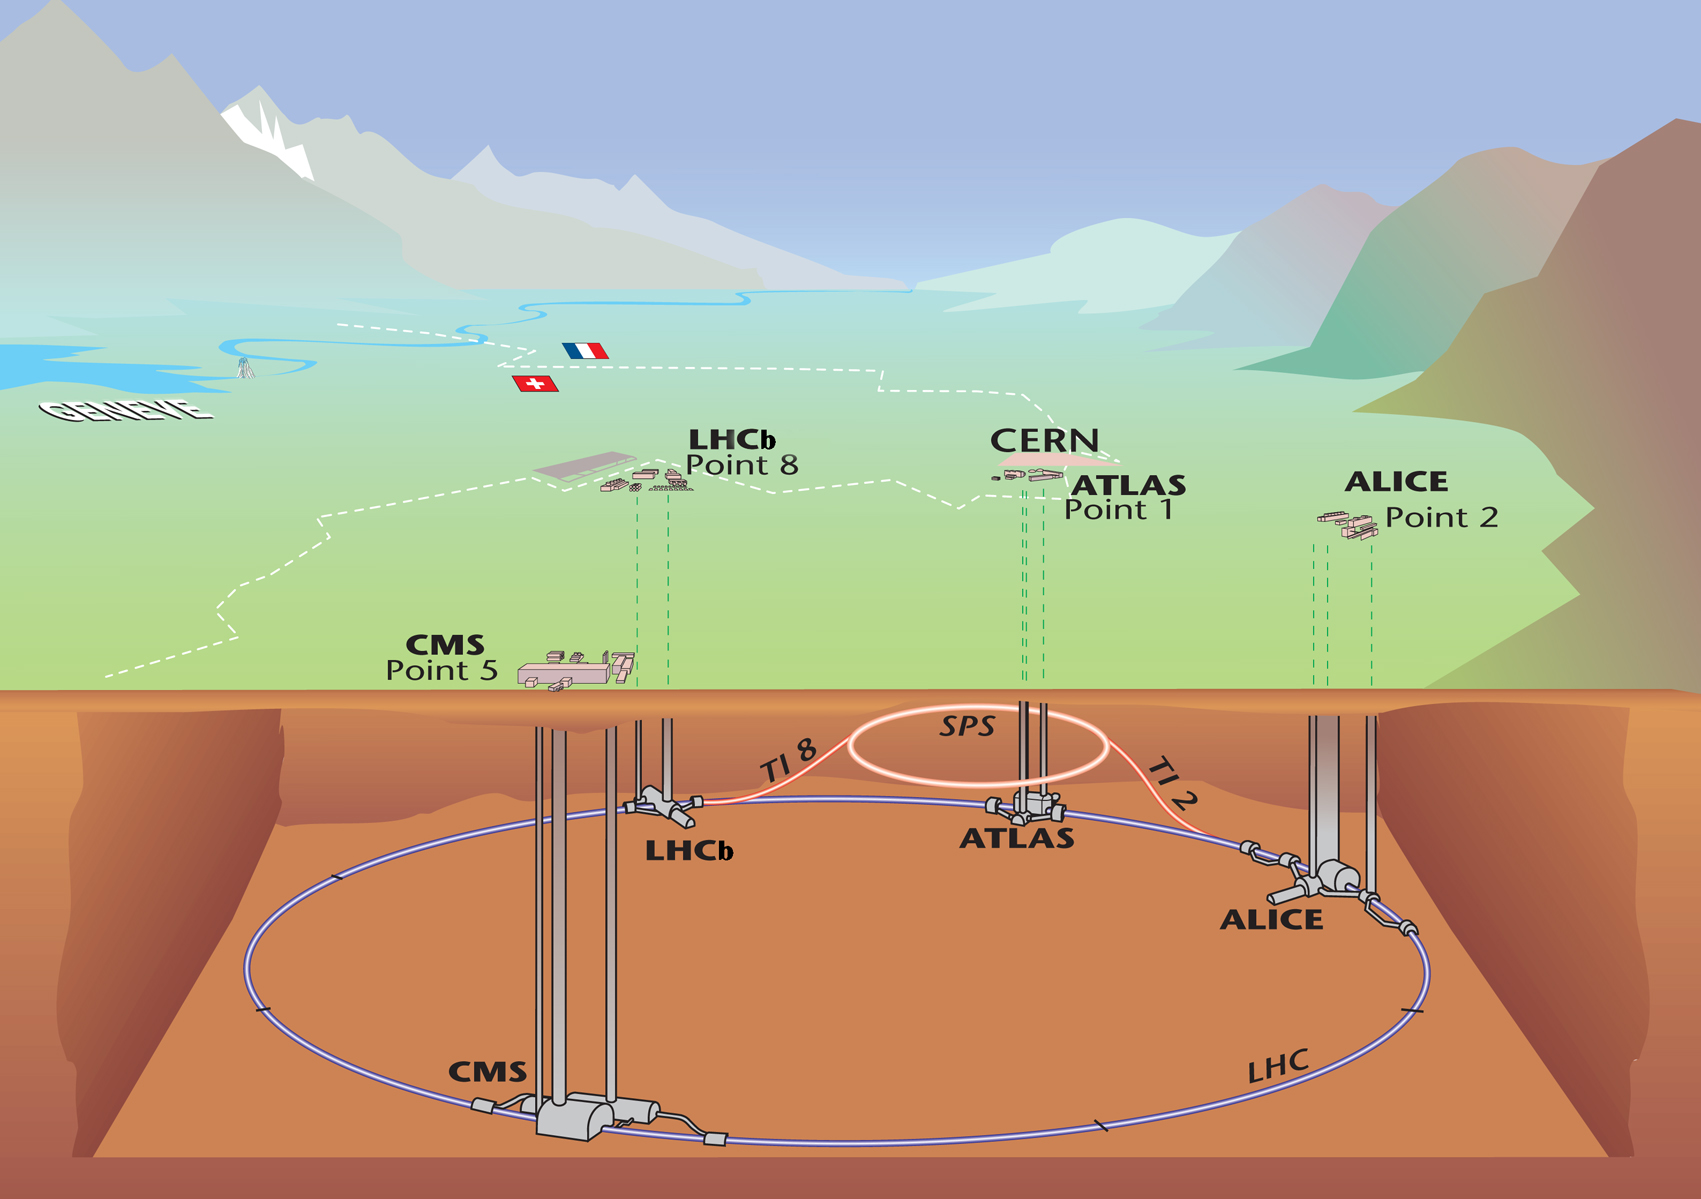
\includegraphics[width=0.9\textwidth]{images/LHC}
  \label{fig:LHC_schematic}
  \caption{Schematic diagram of the Large Hadron Collider, which lies on the border between Switzerland and France. \href{http://cds.cern.ch/journal/CERNBulletin/2008/38/News\%20Articles/1125888?ln=en}{(CERN)}}
\end{figure}

At these colliders, we collide particles at near-lightspeed, creating new particles that can be detected by extremely sophisticated detectors. One of the main challenges at particle colliders is that there are hundreds of millions of particle collisions every second, and only a small fraction of these will have signatures of new physics. That is, the signal is minuscule compared to the background. In addition, there are a multitude of viable theories beyond the Standard Model, with large parameter spaces that can be tested. However, performing a full experimental analysis for a particular search channel can be very time consuming.

For this reason, existing theories must be constrained (or excluded entirely) by holding them up to the light of experimental evidence. Furthermore, we need to have a rough idea of what the most effective collider search strategies are before going ahead with a complete experimental analysis. This is where phenomenology steps in.

Phenomenology bridges the gap between theory and experiment - connecting the predictions of the former with the measurements of the latter. In this dissertation, we describe three phenomenological analyses for finding physics beyond the standard model at current and future colliders, and evaluate their effectiveness. In addition, we describe the potential for machine learning to boost the power of our searches.

In some ways, the progression of the analyses can be viewed as a continuous transition to the greater use of machine learning, as well as higher collider energies. The first analysis described involves searching for light charged Higgs bosons that arise in Two-Higgs doublet models, using a series of rectangular cuts on kinemtical variables that are physically motivated. The second analysis involves a search for heavy higgsinos that decay to a bino-like dark matter candidate. This analysis uses both a series of rectangular cuts on kinmetical variables and a machine learning approach using gradient boosted decision trees. The third analysis (which is still ongoing) forgoes rectangular cuts altogether and uses physically inspired kinematic variables as input features for a machine learning algorithm.
